% 4
%\chapter{${\cal LUTP}$に対するGCNをオラクルとする質問学習モデル}%線形無順序木パターンに対するグラフ畳み込みネットワークをオラクルとする質問学習モデル
\section{${\cal LUTP}$に対するGCNをオラクルとする質問学習モデル}%線形無順序木パターンに対するグラフ畳み込みネットワークをオラクルとする質問学習モデル

%2023年3月2日木曜日から3月4日土曜日まで電気通信大学にて行われた情報処理学会第85回全国大会と,2023年6月29日木曜日から7月1日土曜日まで沖縄科学技術大学院大学カンファレンス・センターにて行われた第143回数理モデル化と問題解決(MPS)と,2024年9月4日水曜日から9月6日金曜日まで広島工業大学五日市キャンパスにて行われた第23回情報科学技術フォーラム(FIT2024)で口頭発表を行った内容である.

% 4.1
\subsection{グラフ畳み込みネットワーク(GCN)}

%\subsection{使用する中間層}
%グラフ構造におけるノード間の情報伝播を実現するための手法であり,隣接行列とその次数行列を用いてノードの特徴量を集約する.GraphConvの主な特徴は,隣接行列を二重に正規化する点にある.このアプローチは,隣接ノードの特徴量を単に加重平均するのではなく,次数の平方根で正規化することによって,グラフ構造をより精緻に反映させることを目的としている.まず,隣接行列を次数行列の逆平方根で左および右に正規化し,その後,隣接ノードの特徴量を加重平均することで,各ノードの新たな特徴量が算出される.この手法は,グラフ上のノードが持つ情報を隣接ノードの情報と効果的に融合させることができるため,グラフの構造を反映した学習が可能となる.GraphConvの計算式は以下のように表される:
\textbf{GCNConv}\footnote{\url{https://pytorch-geometric.readthedocs.io/en/2.5.2/generated/torch_geometric.nn.conv.GCNConv.html}}\cite{pyg-gcnconv}は,頂点の次数に基づく正規化を行うことで,異なる次数を持つ頂点間での特徴ベクトルを正規化する役割を果たす.この正規化により,次数の差異が学習に与える影響を軽減し,頂点間の関係性をより適切に反映した特徴抽出が可能となる.これにより,グラフ全体にわたる情報の伝播が効率的に行われるよう設計されている.式(\ref{eq:gcnconv})に頂点$v$の特徴ベクトル$x_v$を更新するグラフ畳み込み層GCNConvの計算式を示す.ここで,$\textbf{A}$を頂点数$n$~$(n\geq 1)$の入力グラフの隣接行列とする.$\hat{\textbf{A}}=\textbf{A}+\textbf{I}$は,自己ループを持つ隣接行列を表し,$\hat{\textbf{D}}$は,$\hat{D}_{ij}=\sum_{k=1}^{n}\hat{A}_{ik}$~$(i=j)$,$\hat{D}_{ij}=0$~$(i\not=j)$である対角次数行列を表す.ただし,$\hat{A}_{ij}$と$\hat{D}_{ij}$はそれぞれ$\hat{\textbf{A}}$と$\hat{\textbf{D}}$の$(i,j)$成分を表す.すなわち,$\hat{\textbf{D}}^{-\frac{1}{2}}\hat{\textbf{A}}\hat{\textbf{D}}^{-\frac{1}{2}}$で正規化が行われる.
\begin{equation}
  \label{eq:gcnconv}
  \bm{x}'_{v} = \hat{\textbf{D}}^{-\frac{1}{2}}\hat{\textbf{A}}\hat{\textbf{D}}^{-\frac{1}{2}}\bm{x}_{v}\Theta.
\end{equation}

\textbf{GraphConv}\footnote{\url{https://pytorch-geometric.readthedocs.io/en/2.5.3/generated/torch_geometric.nn.conv.GraphConv.html}}\cite{pyg-graphconv}は,特徴量を隣接頂点と自己ループから集約して更新する.つまり,全ての隣接頂点の特徴ベクトルは単純な和として計算される.そのため,頂点の次数が高いほど,より多くの情報を集約することになる.この手法により,次数の影響がそのまま情報集約の範囲に反映され,頂点の重要度に基づいた学習が行われる.式(\ref{eq:graphconv})に頂点$v$の特徴ベクトル$x_v$を更新するグラフ畳み込み層GraphConvの計算式を示す.ここで,$x'_v$は更新した特徴ベクトルを,$\textbf{W}_1,\textbf{W}_2$は重み行列を,$N(v)$は頂点$v$における隣接頂点の集合を表す.また,$e_{\{u,v\}}$は辺$\{u,v\}$に与えられた数値を表す.
\begin{equation}
  \label{eq:graphconv}
  \bm{x}'_{v}=\textbf{W}_{1}\bm{x}_{v}+\textbf{W}_{2}\sum_{v'\in N(v)}e_{\{u,v\}}\bm{x}_{u}.
\end{equation}

\textbf{RGCNConv}\footnote{\url{https://pytorch-geometric.readthedocs.io/en/2.6.1/generated/torch_geometric.nn.conv.RGCNConv.html}}\cite{pyg-rgcnconv}は,関係性を特徴としてGCNConvを拡張した手法である.$R$を辺ラベルの集合とする.ここでは辺ラベルが関係性を表すとする.各辺ラベル$r\in R$に対して専用の重み行列を持つことが特徴である.辺ラベルごとに異なる重み行列を使用し,特徴量を集約して更新することにより,新たな特徴ベクトルを生成する.この過程により,異なる関係性に基づく意味的な差異を捉えることができ,関係性ごとに情報を適切に集約することが可能となる.式(\ref{eq:rgcnconv})に頂点$v$の特徴ベクトル$x_v$を更新するグラフ畳み込み層RGCNConvの計算式を示す.ここで,$x'_v$は更新した特徴ベクトルを,$\textbf{W}_1,\textbf{W}_r$~$(r\in R)$は重み行列を,$N_r(v)$は頂点$v$における辺ラベル$r\in R$ごとに異なる隣接頂点の集合を表す.
\begin{equation}
  \label{eq:rgcnconv}
  \bm{x}'_{v}=\textbf{W}_{1}\bm{x}_{v}+\sum_{r\in R}\left(\sum_{v'\in N_{r}(v)}\frac{1}{|N_{r}(v)|}\textbf{W}_{r}\bm{x}_{v'}\right).
\end{equation}

% 4.2
\subsection{GCNをオラクルとする線形無順序木パターンに対する所属性質問}
線形無順序木パターン$t_*$を目標概念(学習目標)とする.$t_*$において,その所属性質問に正確に回答する完全な教師(オラクル)を${\cal O}(t_{\ast})$と書く.${\cal O}(t_*)$をオラクルとする質問学習モデルを${\cal LUTP}$-${\cal QUERY}_{{\cal O}(t_{\ast})}$とする.${\cal LUTP}$-${\cal QUERY}_{{\cal O}(t_{\ast})}$において,無順序木$T\in{\cal LUTP}$が$T\in L(t_{\ast})$を満たす場合,$T$を$t_{\ast}$の正例と呼び,それ以外の場合を負例と呼ぶ.${\cal LUTP}$-${\cal QUERY}_{{\cal O}(t_{\ast})}$では$L(t_*)$に関する質問に対して正確に回答するオラクル${\cal O}(t_{\ast})$に問い合わせを行うことができる.さらに,$S_{+}\subseteq L(t_{\ast})$と$S_{-}\cap L(t_{\ast})=\emptyset$を満たす無順序木の集合$S_+$と$S_-$が存在すれば,$S_{+}\subseteq L(t)$と$S_{-}\cap L(t)=\emptyset$を満たす線形無順序木パターン$t$が必ず存在する.${\cal O}(t_{\ast})$は無順序木$T$が$L(t_{\ast})$に含まれている場合``$Yes$''を返し,そうでない場合には``$No$''を返す.すなわち,無順序木$T$の所属性質問に対する${\cal O}(t_{\ast})$の回答を${\cal O}(t_{\ast})(T)$で表すとき,${\cal O}(t_{\ast})(T)\in\{Yes,\,No\}$となる(図\ref{fig:ql_oracle}参照).学習目標$L(t_*)$に対して,質問学習アルゴリズム${\cal A}$が$L(t)=L(t_*)$を満たす$t\in {\cal LUTP}$を出力するとき,質問学習アルゴリズム${\cal A}$は$L(t_*)$を同定したという.

% 図4.1
\begin{figure}[tb]
  \centering
  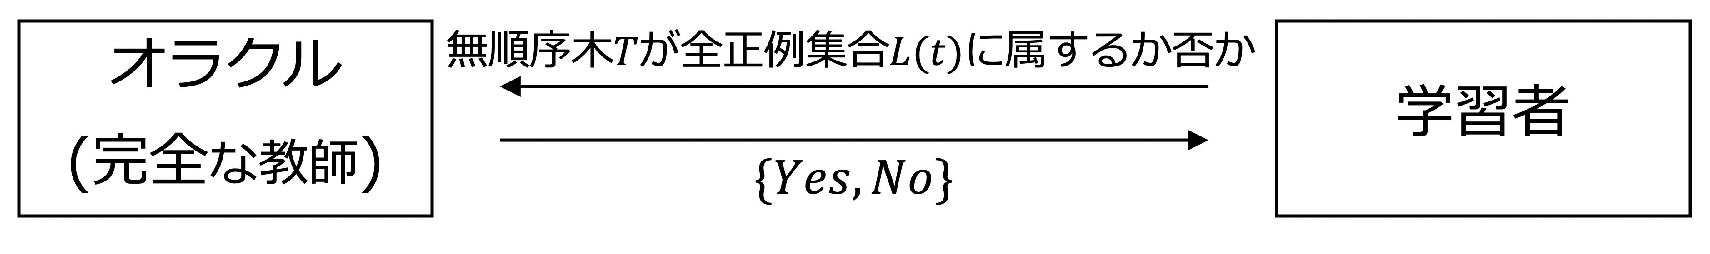
\includegraphics[scale=0.29]{fig-ql_oracle.eps}
  \caption{線形無順序木パターンに対する所属性質問}\label{fig:ql_oracle}
\end{figure}

データセット$S$で学習したGCNを$GCN^S$とするとき,$GCN^S$をオラクルとする質問学習モデルを${\cal LUTP}$-${\cal QUERY}_{GCN^S}$とする.これは,質問学習の一連のプロセスにおいて,${\cal O}(t_{\ast})$を$GCN^S$に置き換え,GCNを活用して学習を協調的に進めるモデルである.これは無順序木を識別するための新しい形式のオラクルとして機能する.${\cal LUTP}$-${\cal QUERY}_{GCN^S}$でも,${\cal LUTP}$-${\cal QUERY}_{{\cal O}(t_{\ast})}$と同様に,正例の無順序木$T\in {\cal LUTP}$を入力とするとき,無順序木パターン$t$が1つだけ出力される.ただし,${\cal LUTP}$-${\cal QUERY}_{GCN^S}$は,不完全な教師であるため,$L(t_{\ast})=L(t)$となる無順序木パターン$t\in{\cal LUTP}$の同定に至らない可能性があることに注意する(図\ref{fig:ql_gcn}参照).

% 図4.2
\begin{figure}[tb]
  \centering
  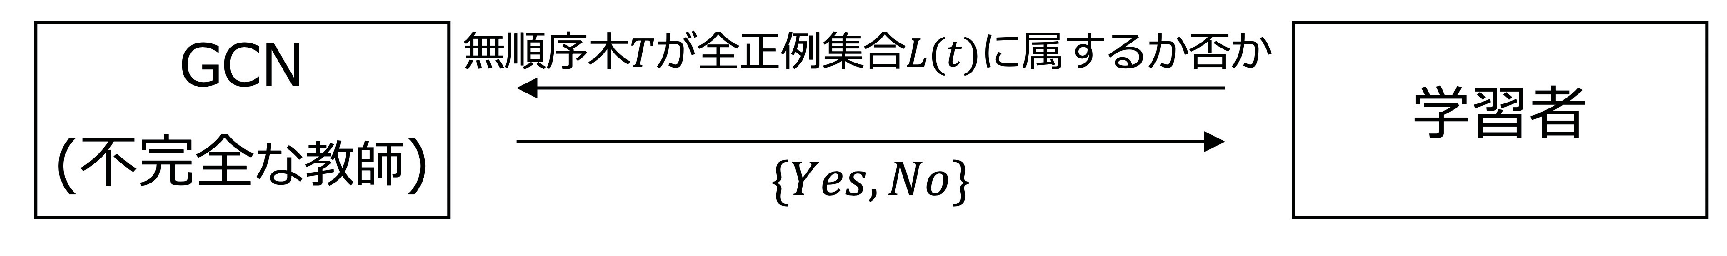
\includegraphics[scale=0.29]{fig-ql_gcn.eps}
  \caption{GCNをオラクルとする線形無順序木パターンに対する所属性質問}\label{fig:ql_gcn}
\end{figure}

% 4.3
\subsection{実験的評価}
混同行列は,機械学習の分類問題において多く使われている評価指標で,TP(True Positive),FP(False Positive),FN(False Negative),TN(True Negative)を実際の値に対する予測の値の結果より分類される結果の値で表される.具体的には,各項\ref{subsec4.3.1}, \ref{subsec4.3.2}, \ref{subsec4.3.3}において定義する.

\textbf{再現率(recall)}とは,真の正例を正しく正例と予測した割合のことで,式(\ref{recall})で計算する.また,\textbf{適合率(precision)}とは,正例と予測したデータのうち真の正例の割合のことで,式(\ref{precision})で計算する.
\begin{equation}
  \label{recall}
  Recall=\frac{TP}{TP+FN},
\end{equation}
\begin{equation}
  \label{precision}
  Precision=\frac{TP}{TP+FP}.
\end{equation}

\textbf{F値(F1-score)}とは,再現率と適合率の調和平均である.F値は式(\ref{f1score})で計算する.本論文では,データセットの分類問題の評価指標としてF値を用いる.
\begin{equation}
  \label{f1score}
  F1 score=\frac{2\times Precision\times Recall}{Precicion+Recall}.
\end{equation}


% 4.3.1
\subsubsection{二値分類問題}\label{subsec4.3.1}
$S_+$と$S_-$を無順序木の集合とする.ただし,$S_+\cap S_-=\emptyset$と仮定する.$S_+^G$と$S_-^G$を$GCN^S$が$S$の無順序木をそれぞれ$S_+$と$S_-$に属すと予測した無順序木の集合とする.学習済みGCNの分類精度を$F$値($F_G$)で評価する.ここで,$TP=|S_+\cap S_+^G|$, $FP=|S_-\cap S_+^G|$, $FN=|S_+\cap S_-^G|$, $TN=|S_-\cap S_-^G|$である.これらを用いて,二値分類問題の再現率,適合率,$F$値をそれぞれ式(\ref{recallg}),(\ref{precisiong}),(\ref{f1scoreg})で算出する.
\begin{equation}
  \label{recallg}
  Recall_G=\frac{|S_+\cap S_+^G|}{|S_+|},
\end{equation}
\begin{equation}
  \label{precisiong}
  Precision_G=\frac{|S_+\cap S_+^G|}{|S_+^G|},
\end{equation}
\begin{equation}
  \label{f1scoreg}
  F_G=\frac{2\times Precision_G\times Recall_G}{Precision_G+Recall_G}.
\end{equation}


% 4.3.2
\subsubsection{無矛盾性問題}\label{subsec4.3.2}
$S_+$と$S_-$を次の条件を満たす${\cal UTP}_{\Sigma,\Lambda,X}$の有限部分集合とする:
無順序木パターン$t_{\ast}\in {\cal LUTP}_{\Sigma,\Lambda,X}$が存在して,$S_+\subset L(t_{\ast})$かつ$S_-\cap L(t_{\ast})=\emptyset$ である.ここでは,NP完全である${\cal LUTP}$-${\cal CP}$の計算問題として,$S_+\subset L(t)$かつ$S_-\cap L(t)=\emptyset$を満たす無順序木パターン$t$を出力する問題を考える.

無順序木$T\in S_+$に対して,${\cal LUTP}$-${\cal QUERY}_{GCN^S}(T)$の出力を$t_T$とする.$S_{+}^{Q(T)}=S\cap L(t_T)$,$S_{-}^{Q(T)}=S\setminus L(t_T)$とする.無順序木パターン$t_T$の精度を$F$値($F_{Q(T)}$)で評価する.ここで,$TP=|S_+\cap S_+^{Q(T)}|$, $FP=|S_-\cap S_+^{Q(T)}|$, $FN=|S_+\cap S_-^{Q(T)}|$, $TN=|S_-\cap S_-^{Q(T)}|$である.これらを用いて,無矛盾性問題の再現率,適合率,$F$値をそれぞれ式(\ref{recallq}),(\ref{precisionq}),(\ref{f1scoreq})で算出する.
\begin{equation}
  \label{recallq}
  Recall_{Q(T)}=\frac{|S_+\cap S_{+}^{Q(T)}|}{|S_+|},
\end{equation}
\begin{equation}
  \label{precisionq}
  Precision_{Q(T)}=\frac{|S_+\cap S_{+}^{Q(T)}|}{|S_{+}^{Q(T)}|},
\end{equation}
\begin{equation}
  \label{f1scoreq}
  F_{Q(T)}=\frac{2\times Precision_{Q(T)}\times Recall_{Q(T)}}{Precision_{Q(T)}+Recall_{Q(T)}}.
\end{equation}

\noindent
最後に式(\ref{fqmax})を達成する無順序木パターン$t$を出力する.
\begin{equation}
  \label{fqmax}
  F_Q=\max_{T\in S_+}F_{Q(T)}.
\end{equation}


% 4.3.3
\subsubsection{可視化問題}\label{subsec4.3.3}
$GCN^S$の可視化としての本手法の精度を,新たに生成した無順序木データ${S'}={S'}_+\cup {S'}_-$ $({S'}_+\cap {S'}_-=\emptyset)$を用いて,$F$値($F'_{GQ}$)で評価する.${S'}_+^G$と${S'}_-^G$を$GCN^S$が$S'$の無順序木をそれぞれ${S'}_+$と${S'}_-$に属すと予測した無順序木の集合とする.式(\ref{fqmax})を達成する無順序木パターン$t$に対して,${S'}_+^Q=S'\cap L(t)$,${S'}_-^Q=S'\setminus L(t)$とする.ここで,$TP=|{S'}_+^{G}\cap {S'}_+^{Q}|$, $FP=|{S'}_-^{G}\cap {S'}_+^{Q}|$, $FN=|{S'}_+^{G}\cap {S'}_-^{Q}|$, $TN=|{S'}_-^{G}\cap {S'}_-^{Q}|$である.これらを用いて,可視化問題の再現率,適合率,$F$値をそれぞれ式(\ref{recallgq}),(\ref{precisiongq}),(\ref{f1scoregq})で算出する.
\begin{equation}
  \label{recallgq}
  Recall'_{GQ}=\frac{|{S'}_+^G\cap {S'}_+^Q|}{|{S'}_+^G|},
\end{equation}
\begin{equation}
  \label{precisiongq}
  Precision'_{GQ}=\frac{|{S'}_+^G\cap {S'}_+^Q|}{|{S'}_+^Q|},
\end{equation}
\begin{equation}
  \label{f1scoregq}
  F'_{GQ}=\frac{2\times Precision'_{GQ}\times Recall'_{GQ}}{Precision'_{GQ}+Recall'_{GQ}}.
\end{equation}


% 4.4
\subsection{協調モデルの解析}
実験手順をアルゴリズム\ref{alg:exp_ql-gcn}に示す.計算機実験では,$\abs{S_+}=5000, \abs{S_-}=5000, \abs{S_L}=6400, \abs{S_V}=1600, \abs{S_T}=2000, \abs{S'}=10000$とし,この条件下で実験を行った.実験では,グラフ畳み込み層として(1)\,GraphConv,(2)\,RGCNConv,(3)\,GCNConvを使用し,質問学習アルゴリズムとして(a)\,${\cal LUTP}$-${\cal QUERY}_{GCN^S}^{Linear}$,(b)\,${\cal LUTP}$-${\cal QUERY}_{GCN^S}^{Square}$をそれぞれ使用し,これらの全ての組み合わせに対して計算機実験を実施した.それぞれ5487回の試行を繰り返し,安定した結果を得るようにした.GCNの学習においては,無順序木の各頂点$v$に与える初期の特徴ベクトルを,以下の7つの特徴量から構成した.

\begin{enumerate}
  \item[(i)] $v$の根からの深さ,
  \item[(ii)] $v$の子の数,
  \item[(iii)] $v$の子孫の数($v$から深さ2まで),
  \item[(iv)]$v$の子孫の数($v$から深さ3まで),
  \item[(v)] $v$の子孫の数($v$から深さ4まで),
  \item[(vi)] $v$の子孫の数,
  \item[(vii)] $v$の親への辺ラベルのone-hotベクトル,ただし,辺ラベル集合は$\Lambda=\{a,b,c,d,e\}$とする.
\end{enumerate}

% アルゴリズム8
\begin{algorithm}[tb]
\caption{GCNをオラクルとする質問学習(${\cal LUTP}$-${\cal QUERY}_{GCN^S}$)の実験手順;} \label{alg:exp_ql-gcn}
\begin{algorithmic}[1]
  \Require{$t_{\ast}\in {\cal LUTP}$;}
  \State $S\coloneqq S_+\cup S_-~(S_+\subset L(t_{\ast})\land S_-\cap L(t_{\ast})=\emptyset)$を生成;
  \State $GCN^S\coloneqq S$を学習データ$S_L$,検証データ$S_V$,テストデータ$S_T$に分割し$GCN^S$を構築;
  \State $Rec=\frac{|{S}_+\cap {S}_+^G|}{|{S}_+|}$,
      $Prec=\frac{|{S}_+\cap {S}_+^G|}{|{S}_+^G|}$,
      $F_G=\frac{2\times Prec\times Rec}{Prec+Rec}$;
  \For{$T\in S_+$}
    \State $t_T\coloneqq {\cal LUTP}$-${\cal QUERY}_{GCN^S}^{Linear}(T)$の出力;
    \State $Rec=\frac{|S_+\cap S_{+}^{Q_{Linear}(t_T)}|}{|S_+|}$,
    $Prec=\frac{|S_+\cap S_{+}^{Q_{Linear}(t_T)}|}{|S_{+}^{Q_{Linear}(t_T)}|}$,
    $F_{Q_{Linear}(t_T)}=\frac{2\times Prec\times Rec}{Prec+Rec}$;
    \State $t_T\coloneqq {\cal LUTP}$-${\cal QUERY}_{GCN^S}^{Square}(t_T)$の出力;
    \State $Rec=\frac{|S_+\cap S_{+}^{Q_{Square}(t_T)}|}{|S_+|}$,
    $Prec=\frac{|S_+\cap S_{+}^{Q_{Square}(t_T)}|}{|S_{+}^{Q_{Square}(t_T)}|}$,
    $F_{Q_{Square}(t_T)}=\frac{2\times Prec\times Rec}{Prec+Rec}$;
  \EndFor
  \State $F_{Q_{Linear}}\coloneqq \max_{T\in S_+}F_{Q(T)_{Linear}}$, $F_{Q_{Square}}\coloneqq \max_{T\in S_+}F_{Q(T)_{Square}}$;
  \State $t_{Linear}\coloneqq F_{Q_{Linear}}$を達成する無順序木パターン;
  \State $t_{Square}\coloneqq F_{Q_{Square}}$を達成する無順序木パターン;

  \State $S'\coloneqq S'_+\cup S'_-~(S'_+\subset L(t_{\ast})\land S'_-\cap L(t_{\ast})=\emptyset)$を生成;
  \State $Recall\coloneqq\frac{|{S'}_+\cap {S'}_+^G|}{|{S'}_+|}$,
      $Precision\coloneqq\frac{|{S'}_+\cap {S'}_+^G|}{|{S'}_+^G|}$,
      $F'_G\coloneqq\frac{2\times Precision\times Recall}{Precision+Recall}$;
    \For{$T\in S'_+$}
      \State $Rec\coloneqq\frac{|{S'}_+\cap {S'}_{+}^{Q_{Linear}(T)}|}{|{S'}_+|}$,
      $Prec\coloneqq\frac{|{S'}_+\cap {S'}_{+}^{Q_{Linear}(T)}|}{|{S'}_{+}^{Q_{Linear}(T)}|}$,
      $F_{Q_{Linear}(T)}\coloneqq\frac{2\times Prec\times Rec}{Prec+Rec}$;
      \State $Rec\coloneqq\frac{|{S'}_+\cap {S'}_{+}^{Q_{Square}(T)}|}{|{S'}_+|}$,
      $Prec\coloneqq\frac{|{S'}_+\cap {S'}_{+}^{Q_{Square}(T)}|}{|{S'}_{+}^{Q_{Square}(T)}|}$,
      $F_{Q_{Square}(T)}\coloneqq\frac{2\times Prec\times Rec}{Prec+Rec}$;
    \EndFor
  \State ${F'}_{Q_{Linear}}\coloneqq\max_{T\in {S'}_+}{F'}_{Q_{Linear}(T)}$;
  \State ${F'}_{Q_{Square}}\coloneqq\max_{T\in {S'}_+}{F'}_{Q_{Square}(T)}$;
  \State $Rec\coloneqq\frac{|{S'}_+^G\cap {S'}_+^{Q_{Linear}}|}{|{S'}_+^G|}$,
  $Prec\coloneqq\frac{|{S'}_+^G\cap {S'}_+^{Q_{Linear}}|}{|{S'}_+^{Q_{Linear}}|}$,
  $F'_{GQ_{Linear}}\coloneqq\frac{2\times Prec\times Rec}{Prec+Rec}$;
  \State $Rec\coloneqq\frac{|{S'}_+^G\cap {S'}_+^{Q_{Square}}|}{|{S'}_+^G|}$,
  $Prec\coloneqq\frac{|{S'}_+^G\cap {S'}_+^{Q_{Square}}|}{|{S'}_+^{Q_{Square}}|}$,
  $F'_{GQ_{Square}}\coloneqq\frac{2\times Prec\times Rec}{Prec+Rec}$;
\end{algorithmic}
\end{algorithm}

%実験結果を示す.
グラフ畳み込み層にGraphConvを使用した実験結果を図\ref{fig:result_graphconv}と表\ref{tbl:result_graphconv}に,RGCNConvを使用した実験結果を図\ref{fig:result_rgcnconv}と表\ref{tbl:result_rgcnconv}に,GCNConvを使用した実験結果を図\ref{fig:result_gcnconv}と表\ref{tbl:result_gcnconv}に示す.

% 図4.3
\begin{figure*}[tb]
  \centering
  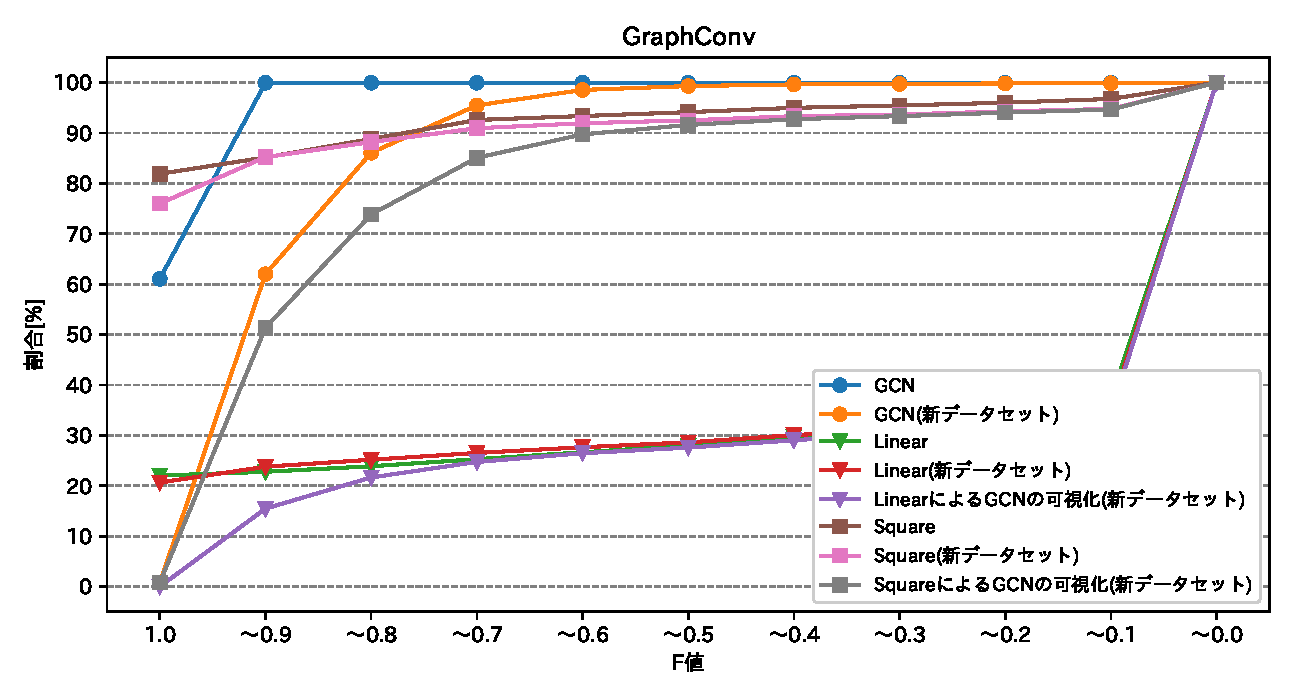
\includegraphics[scale=0.7]{fig-exp_GraphConv.eps}
  \caption{横軸のF値超を達成した実験の割合(GraphConv)}\label{fig:result_graphconv}
\end{figure*}

% 表4.1
\begin{table*}[tb]
\caption{GraphConvの分類精度}\label{tbl:result_graphconv}
\centering
\begin{tabular}{|c|r|r|r|r|r|r|r|r|}\hline
  & \multicolumn{1}{|c|}{$F_{G}$} & \multicolumn{1}{|c|}{$F_{Q_{Linear}}$} & \multicolumn{1}{|c|}{$F_{Q_{Square}}$} & \multicolumn{1}{|c|}{$F'_{G}$} & \multicolumn{1}{|c|}{${F'}_{Q_{Linear}}$} & \multicolumn{1}{|c|}{${F'}_{Q_{Square}}$} & \multicolumn{1}{|c|}{${F'}_{GQ_{Linear}}$} & \multicolumn{1}{|c|}{${F'}_{GQ_{Square}}$}\\
  \hline
  \multicolumn{1}{|c|}{F値} & \multicolumn{1}{|c|}{割合} & \multicolumn{1}{|c|}{割合} & \multicolumn{1}{|c|}{割合} & \multicolumn{1}{|c|}{割合} & \multicolumn{1}{|c|}{割合} & \multicolumn{1}{|c|}{割合} & \multicolumn{1}{|c|}{割合} & \multicolumn{1}{|c|}{割合} \\
  \hline
  1.0   & 61.1 & 22.0 & 81.9 & 0.8 & 20.6 & 76.0 & 0.0 & 0.8 \\
  〜0.9 & 100.0 & 22.8 & 85.1 & 62.0 & 23.8 & 85.2 & 15.5 & 51.4 \\
  〜0.8 & 100.0 & 23.9 & 88.8 & 86.1 & 25.2 & 88.2 & 21.7 & 73.8 \\
  〜0.7 & 100.0 & 25.3 & 92.6 & 95.5 & 26.5 & 90.9 & 24.7 & 85.1 \\
  〜0.6 & 100.0 & 26.6 & 93.4 & 98.5 & 27.6 & 91.9 & 26.5 & 89.7 \\
  〜0.5 & 100.0 & 28.0 & 94.1 & 99.3 & 28.6 & 92.5 & 27.6 & 91.6 \\
  〜0.4 & 100.0 & 29.8 & 95.0 & 99.6 & 30.1 & 93.3 & 29.0 & 92.7 \\
  〜0.3 & 100.0 & 31.3 & 95.5 & 99.7 & 31.1 & 93.7 & 30.5 & 93.3 \\
  〜0.2 & 100.0 & 33.0 & 96.0 & 99.8 & 32.1 & 94.3 & 31.8 & 94.0 \\
  〜0.1 & 100.0 & 37.3 & 96.8 & 99.9 & 35.4 & 94.8 & 34.5 & 94.7 \\
  〜0.0 & 100.0 & 100.0 & 100.0 & 100.0 & 100.0 & 100.0 & 100.0 & 100.0 \\
  \hline
\end{tabular}
\end{table*}

% 図4.4
\begin{figure*}[tb]
  \centering
  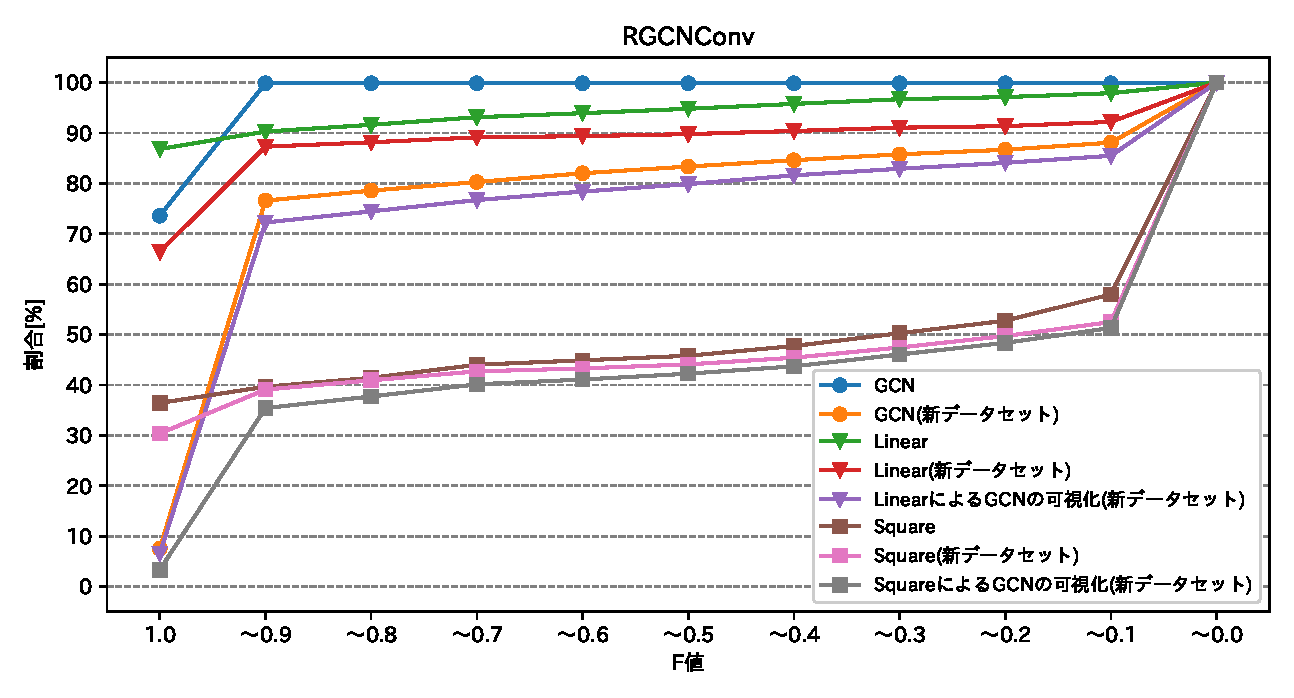
\includegraphics[scale=0.7]{fig-exp_RGCNConv.eps}
  \caption{横軸のF値超を達成した実験の割合(RGCNConv)}\label{fig:result_rgcnconv}
\end{figure*}

% 表4.2
\begin{table*}[tb]
\caption{RGCNConvの分類精度}\label{tbl:result_rgcnconv}
\centering
\begin{tabular}{|c|r|r|r|r|r|r|r|r|}\hline
  & \multicolumn{1}{|c|}{$F_{G}$} & \multicolumn{1}{|c|}{$F_{Q_{Linear}}$} & \multicolumn{1}{|c|}{$F_{Q_{Square}}$} & \multicolumn{1}{|c|}{$F'_{G}$} & \multicolumn{1}{|c|}{${F'}_{Q_{Linear}}$} & \multicolumn{1}{|c|}{${F'}_{Q_{Square}}$} & \multicolumn{1}{|c|}{${F'}_{GQ_{Linear}}$} & \multicolumn{1}{|c|}{${F'}_{GQ_{Square}}$}\\
  \hline
  \multicolumn{1}{|c|}{F値} & \multicolumn{1}{|c|}{割合} & \multicolumn{1}{|c|}{割合} & \multicolumn{1}{|c|}{割合} & \multicolumn{1}{|c|}{割合} & \multicolumn{1}{|c|}{割合} & \multicolumn{1}{|c|}{割合} & \multicolumn{1}{|c|}{割合} & \multicolumn{1}{|c|}{割合} \\
  \hline
  1.0   & 73.6 & 86.8 & 36.4 & 7.5 & 66.4 & 30.4 & 6.5 & 3.3 \\
  〜0.9 & 99.9 & 90.3 & 39.7 & 76.6 & 87.3 & 39.1 & 72.2 & 35.4 \\
  〜0.8 & 99.9 & 91.6 & 41.4 & 78.6 & 88.2 & 40.9 & 74.4 & 37.7 \\
  〜0.7 & 99.9 & 93.1 & 44.0 & 80.3 & 89.1 & 42.7 & 76.7 & 40.1 \\
  〜0.6 & 99.9 & 93.9 & 44.9 & 82.0 & 89.4 & 43.3 & 78.4 & 41.1 \\
  〜0.5 & 99.9 & 94.8 & 45.8 & 83.3 & 89.8 & 44.1 & 79.9 & 42.2 \\
  〜0.4 & 99.9 & 95.8 & 47.7 & 84.6 & 90.4 & 45.4 & 81.6 & 43.7 \\
  〜0.3 & 99.9 & 96.7 & 50.3 & 85.8 & 91.1 & 47.4 & 82.9 & 46.1 \\
  〜0.2 & 99.9 & 97.1 & 52.7 & 86.7 & 91.4 & 49.7 & 84.1 & 48.4 \\
  〜0.1 & 99.9 & 97.9 & 58.0 & 88.1 & 92.2 & 52.5 & 85.5 & 51.3 \\
  〜0.0 & 100.0 & 100.0 & 100.0 & 100.0 & 100.0 & 100.0 & 100.0 & 100.0 \\
  \hline
\end{tabular}
\end{table*}

% 図4.5
\begin{figure*}[tb]
  \centering
  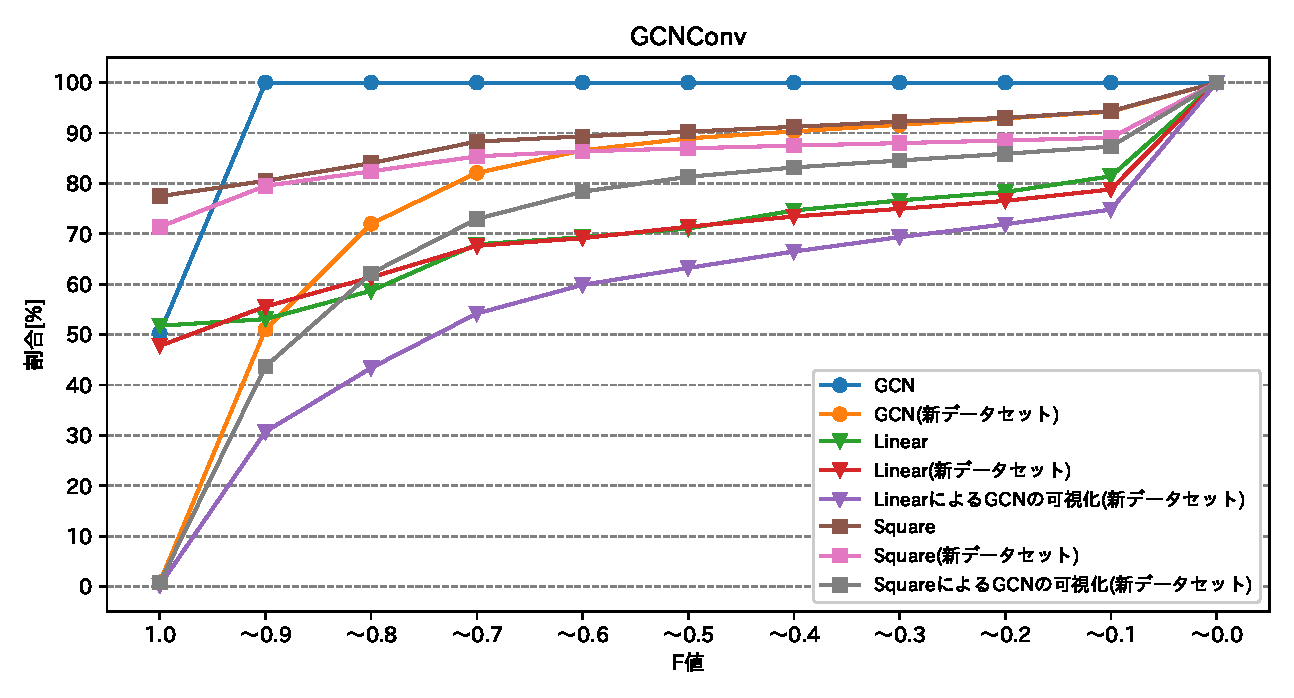
\includegraphics[scale=0.7]{fig-exp_GCNConv.eps}
  \caption{横軸のF値超を達成した実験の割合(GCNConv)}\label{fig:result_gcnconv}
\end{figure*}

% 表4.3
\begin{table*}[tb]
\caption{GCNConvの分類精度}\label{tbl:result_gcnconv}
\centering
\begin{tabular}{|c|r|r|r|r|r|r|r|r|}\hline
  & \multicolumn{1}{|c|}{$F_{G}$} & \multicolumn{1}{|c|}{$F_{Q_{Linear}}$} & \multicolumn{1}{|c|}{$F_{Q_{Square}}$} & \multicolumn{1}{|c|}{$F'_{G}$} & \multicolumn{1}{|c|}{${F'}_{Q_{Linear}}$} & \multicolumn{1}{|c|}{${F'}_{Q_{Square}}$} & \multicolumn{1}{|c|}{${F'}_{GQ_{Linear}}$} & \multicolumn{1}{|c|}{${F'}_{GQ_{Square}}$}\\
  \hline
  \multicolumn{1}{|c|}{F値} & \multicolumn{1}{|c|}{割合} & \multicolumn{1}{|c|}{割合} & \multicolumn{1}{|c|}{割合} & \multicolumn{1}{|c|}{割合} & \multicolumn{1}{|c|}{割合} & \multicolumn{1}{|c|}{割合} & \multicolumn{1}{|c|}{割合} & \multicolumn{1}{|c|}{割合} \\
  \hline
  1.0   & 50.2 & 51.8 & 77.5 & 0.9 & 47.8 & 71.4 & 0.2 & 0.8 \\
  〜0.9 & 100.0 & 53.1 & 80.5 & 51.0 & 55.6 & 79.5 & 30.7 & 43.7 \\
  〜0.8 & 100.0 & 58.7 & 84.0 & 72.0 & 61.4 & 82.4 & 43.4 & 62.1 \\
  〜0.7 & 100.0 & 67.9 & 88.3 & 82.1 & 67.6 & 85.4 & 54.2 & 72.9 \\
  〜0.6 & 100.0 & 69.3 & 89.3 & 86.6 & 69.1 & 86.4 & 59.9 & 78.3 \\
  〜0.5 & 100.0 & 71.0 & 90.3 & 88.9 & 71.4 & 87.0 & 63.2 & 81.3 \\
  〜0.4 & 100.0 & 74.6 & 91.2 & 90.3 & 73.4 & 87.5 & 66.5 & 83.2 \\
  〜0.3 & 100.0 & 76.6 & 92.3 & 91.6 & 75.0 & 88.0 & 69.3 & 84.5 \\
  〜0.2 & 100.0 & 78.3 & 93.0 & 92.9 & 76.5 & 88.5 & 71.9 & 85.9 \\
  〜0.1 & 100.0 & 81.4 & 94.3 & 94.2 & 78.8 & 89.1 & 74.8 & 87.3 \\
  〜0.0 & 100.0 & 100.0 & 100.0 & 100.0 & 100.0 & 100.0 & 100.0 & 100.0 \\
  \hline
\end{tabular}
\end{table*}

%% 結果・考察
\subsection{協調モデルの解析に関する考察}
%$F$値の評価基準として,0.9を超えれば高精度,0.1以下であれば低精度とみなす.
%結果より,GraphConvに関して,高精度で分類することのできる線形無順序木パターンを,${\cal LUTP}$-${\cal QUERY}_{GCN^S}^{Linear}$では全実験5487回のうち22.8\%,${\cal LUTP}$-${\cal QUERY}_{GCN^S}^{Square}$では85.1\%の割合で発見することができた.一方で,RGCNConvに関して高精度で分類することのできる線形無順序木パターンを,${\cal LUTP}$-${\cal QUERY}_{GCN^S}^{Linear}$では90.3\%,${\cal LUTP}$-${\cal QUERY}_{GCN^S}^{Square}$では39.7\%の割合で発見することができた.このことから,GraphConvは${\cal LUTP}$-${\cal QUERY}_{GCN^S}^{Square}$を得意とし,RGCNConvは${\cal LUTP}$-${\cal QUERY}_{GCN^S}^{Linear}$を得意とすることが確認できる.これは,GraphConvは近接する頂点間の特徴,RGCNConvは同じ辺ラベルの特徴を捉えているからであると考えられる.
%
%次に学習の際に使用したデータセット$S$と新しいデータセット$S'$の比較を行う.精度の高かった(GraphConv, ${\cal LUTP}$-${\cal QUERY}_{GCN^S}^{Square}$),(RGCNConv, ${\cal LUTP}$-${\cal QUERY}_{GCN^S}^{Linear}$)ともに$F_G=1.0$であった実験の割合と$F'_G=1.0$の割合の差が著しい.このことから学習済みGCNは過学習を起こしている可能性が高いと言える.一方で,質問学習によって発見された線形無順序木パターンは,どちらのグラフ畳み込み層でも$F_G=1.0$であった実験の割合と$F'_G=1.0$の割合の差が小さい.このことは発見された線形無順序木パターンでは過学習を起こしにくいということを示唆している.過学習を起こしにくいことの理由の一つとして,線形無順序木パターンに対する質問学習モデルが無順序木であることを前提に行われていることがあげられる.
%
%中間層の特徴と使用するアルゴリズムの特徴によって顕著な差があることがわかった.そこで,相関関係について調査を行った.まず,任意のF値以上を達成した線形無順序木パターンの集合を$P$,達成できなかった集合を$N$とし,それぞれの線形無順序木パターンの葉のうち変数である割合を調べた.結果を表\ref{tbl:variable_ratio}に示す.結果より,F値と葉のうち変数である割合の間に相関は見られなかった.

%実験結果を3つの計算問題と照らし合わせてみる.%$F$値の評価基準として,0.9を超えれば高精度,0.1以下であれば低精度とみなすこととする.
\subsubsection*{二値分類問題に関する考察}
二値分類問題に関しては,$F_G$が0.9以上を獲得できた実験が全実験5487回のうち,GraphConvでは100.0\%,RGCNConvでは99.9\%,GCNConvでは100.0\%と,いずれのグラフ畳み込み層を使用した場合においても,非常に高い分類精度が達成されることが確認された.一方で,新しいデータセットでの分類精度$F'_G$は,GraphConvでは62.0\%,RGCNConvでは76.6\%,GCNConvでは51.0\%と大きく低下しており,学習データに依存した過学習が発生している可能性が示唆される.

\subsubsection*{無矛盾性問題に関する考察}
無矛盾性問題に関しては,使用するグラフ畳み込み層と質問学習アルゴリズムの組み合わせによって顕著な差が確認される.GraphConvを使用した場合,$F_{Q_{Linear}}$と$F_{Q_{Square}}$に対して0.9以上を獲得できた実験が全実験5487回のうち,アルゴリズム${\cal LUTP}$-${\cal QUERY}_{GCN^S}^{Linear}$で得られた線形無順序木パターンの分類精度$F_{Q_{Linear}}$は22.8\%にとどまった.一方,${\cal LUTP}$-${\cal QUERY}_{GCN^S}^{Square}$では85.1\%と大幅に高い分類精度$F_{Q_{Square}}$が達成されており,両アルゴリズム間で明確な差が見られる.さらに,図\ref{fig:result_graphconv}全体を確認すると,${\cal LUTP}$-${\cal QUERY}_{GCN^S}^{Linear}$による結果は図の下側を中心に位置している一方,${\cal LUTP}$-${\cal QUERY}_{GCN^S}^{Square}$の結果は図の上側を中心に位置していることがわかる.これらの結果は,GraphConvを用いた場合,アルゴリズム${\cal LUTP}$-${\cal QUERY}_{GCN^S}^{Square}$の方が学習効果が高いことを示している.RGCNConvを使用した場合,アルゴリズム${\cal LUTP}$-${\cal QUERY}_{GCN^S}^{Linear}$で得られた線形無順序木パターンの分類精度$F_{Q_{Linear}}$は90.3\%と非常に高精度である.一方,${\cal LUTP}$-${\cal QUERY}_{GCN^S}^{Square}$では39.7\%と低精度であり,RGCNConvを用いた場合でも両アルゴリズムで明確な差が見られる.さらに,図\ref{fig:result_rgcnconv}全体を確認すると,${\cal LUTP}$-${\cal QUERY}_{GCN^S}^{Linear}$による結果は図の上側を中心に位置している一方,${\cal LUTP}$-${\cal QUERY}_{GCN^S}^{Square}$の結果は図の下側を中心に位置している.これらの結果は,RGCNConvを用いた場合,アルゴリズム${\cal LUTP}$-${\cal QUERY}_{GCN^S}^{Linear}$の方が学習効果が高いことを示している.GCNConvでは,GraphConvやRGCNConvにおけるような大きな差は確認されていない.

\subsubsection*{可視化問題に関する考察}
可視化問題に関しては,無矛盾性問題と同様の傾向が確認される.具体的には,グラフ畳み込み層GraphConvでは,アルゴリズム${\cal LUTP}$-${\cal QUERY}_{GCN^S}^{Square}$の方が高い精度${F'}_{GQ_{Square}}$でGCNの予測根拠を可視化している.一方でRGCNConvでは,${\cal LUTP}$-${\cal QUERY}_{GCN^S}^{Linear}$の方が高い精度${F'}_{GQ_{Linear}}$でGCNの予測根拠を可視化していることが確認された.これらの結果は,GraphConvでは${\cal LUTP}$-${\cal QUERY}_{GCN^S}^{Square}$の方が,RGCNConvでは${\cal LUTP}$-${\cal QUERY}_{GCN^S}^{Linear}$の方が学習効果に優れており,分類精度の高い線形無順序木パターンを獲得することが可能であるため,GCNの予測根拠を可視化できていると考えられる.これらの結果から,GraphConvを使用した場合はアルゴリズム${\cal LUTP}$-${\cal QUERY}_{{\cal O}(t)}^{Square}$の精度が高く,RGCNConvを使用した場合はアルゴリズム${\cal LUTP}$-${\cal QUERY}_{{\cal O}(t)}^{Linear}$の精度が高いことが確認される.この違いは,使用するグラフ畳み込み層の特徴に起因していると考えられる.具体的には,GraphConvが隣接する頂点数に基づいて特徴を集約するのに対し,RGCNConvが辺ラベルの種類に基づいて特徴を集約するという両者の特性の違いがあり,それがGCNの学習効果に影響を与えていると考えられる.

% 表4.4
\begin{table*}[tb]
\caption{F値と変数の割合の関係}\label{tbl:variable_ratio}
\centering
\begin{tabular}{|c|rr|rr|rr|rr|rr|rr|}\hline
  \multicolumn{7}{|c|}{${\cal LUTP}$-${\cal QUERY}_{GCN^S}^{Linear}$} \\ \hline
  \multirow{2}{*}{F値} & \multicolumn{2}{|c|}{GraphConv} & \multicolumn{2}{|c|}{RGCNConv} & \multicolumn{2}{|c|}{GCNConv} \\ \cline{2-7}
  & P: 変数の割合 & N: 変数の割合 & P: 変数の割合 & N: 変数の割合 & P: 変数の割合 & N: 変数の割合 \\ \hline
  0.9 &   0.65479 &       0.44864 &       0.48297 &       0.61297 &       0.51224 &       0.47678 \\
  0.8 &   0.65618 &       0.44524 &       0.48568 &       0.60398 &       0.51343 &       0.47028 \\
  0.7 &   0.65786 &       0.44071 &       0.48811 &       0.59711 &       0.49702 &       0.49260 \\
  0.6 &   0.66183 &       0.43522 &       0.49024 &       0.57854 &       0.50064 &       0.48422 \\
  0.5 &   0.66332 &       0.43046 &       0.49199 &       0.56143 &       0.50260 &       0.47843 \\
  0.4 &   0.66015 &       0.42582 &       0.49272 &       0.56097 &       0.49799 &       0.48857 \\
  0.3 &   0.65904 &       0.42116 &       0.49446 &       0.52904 &       0.49900 &       0.48447 \\
  0.2 &   0.65975 &       0.41460 &       0.49543 &       0.50154 &       0.50081 &       0.47680 \\
  0.1 &   0.64320 &       0.40777 &       0.49629 &       0.46327 &       0.50252 &       0.46532 \\ \hline\hline
  \multicolumn{7}{|c|}{${\cal LUTP}$-${\cal QUERY}_{GCN^S}^{Square}$} \\ \hline
  0.9 &   0.47923 &       0.58944 &       0.44011 &       0.53207 &       0.46454 &       0.62384 \\
  0.8 &   0.48282 &       0.59703 &       0.44477 &       0.53155 &       0.46933 &       0.63387 \\
  0.7 &   0.48665 &       0.60732 &       0.44288 &       0.53705 &       0.47379 &       0.66021 \\
  0.6 &   0.48858 &       0.59438 &       0.44651 &       0.53559 &       0.47669 &       0.65409 \\
  0.5 &   0.48975 &       0.58943 &       0.45066 &       0.53358 &       0.47868 &       0.65255 \\
  0.4 &   0.49037 &       0.59473 &       0.45211 &       0.53532 &       0.47985 &       0.65921 \\
  0.3 &   0.49103 &       0.59171 &       0.45328 &       0.53837 &       0.48193 &       0.65842 \\
  0.2 &   0.49176 &       0.58812 &       0.45463 &       0.54133 &       0.48337 &       0.65775 \\
  0.1 &   0.49282 &       0.57859 &       0.46779 &       0.53397 &       0.48694 &       0.63974 \\ \hline
\end{tabular}
\end{table*}

\subsubsection*{精度と精度以外の相関関係に関する考察}
計算機実験ではランダムに生成した線形無順序木パターンを用いているが,協調モデルによって出力される線形無順序木パターンには精度が高いものと低いものが存在することが確認される.そこで,精度と精度以外の数値の相関関係について調査する.
まず,各F値に対して質問回数の多少について調査を行う.使用したGCNのグラフ畳み込み層と質問アルゴリズムのペアを順序対で表す.(GraphConv, ${\cal LUTP}$-${\cal QUERY}_{GCN^S}^{Linear}$)の結果を図\ref{fig:GraphConv_ln_ql_f1_nodes}に,(GraphConv, ${\cal LUTP}$-${\cal QUERY}_{GCN^S}^{Square}$)の結果を図\ref{fig:GraphConv_sqr_ql_f1_nodes}に,(RGCNConv, ${\cal LUTP}$-${\cal QUERY}_{GCN^S}^{Linear}$)の結果を図\ref{fig:RGCNConv_ln_ql_f1_nodes}に,(RGCNConv, ${\cal LUTP}$-${\cal QUERY}_{GCN^S}^{Square}$)の結果を図\ref{fig:RGCNConv_sqr_ql_f1_nodes}に,(GCNConv, ${\cal LUTP}$-${\cal QUERY}_{GCN^S}^{Linear}$)の結果を図\ref{fig:GCNConv_ln_ql_f1_nodes}に,(GCNConv, ${\cal LUTP}$-${\cal QUERY}_{GCN^S}^{Square}$)の結果を図\ref{fig:GCNConv_sqr_ql_f1_nodes}に示す.いずれの結果もF値と質問回数の間に相関は見られない.さらに,正例の総頂点数を加えて調査する.この調査では,質問回数と頂点数の間に正の相関が見られる.これは,正例の頂点数が質問回数に影響を与えることであり,自明な結果である.

% 図4.6
\begin{figure*}[tb]
  \centering
  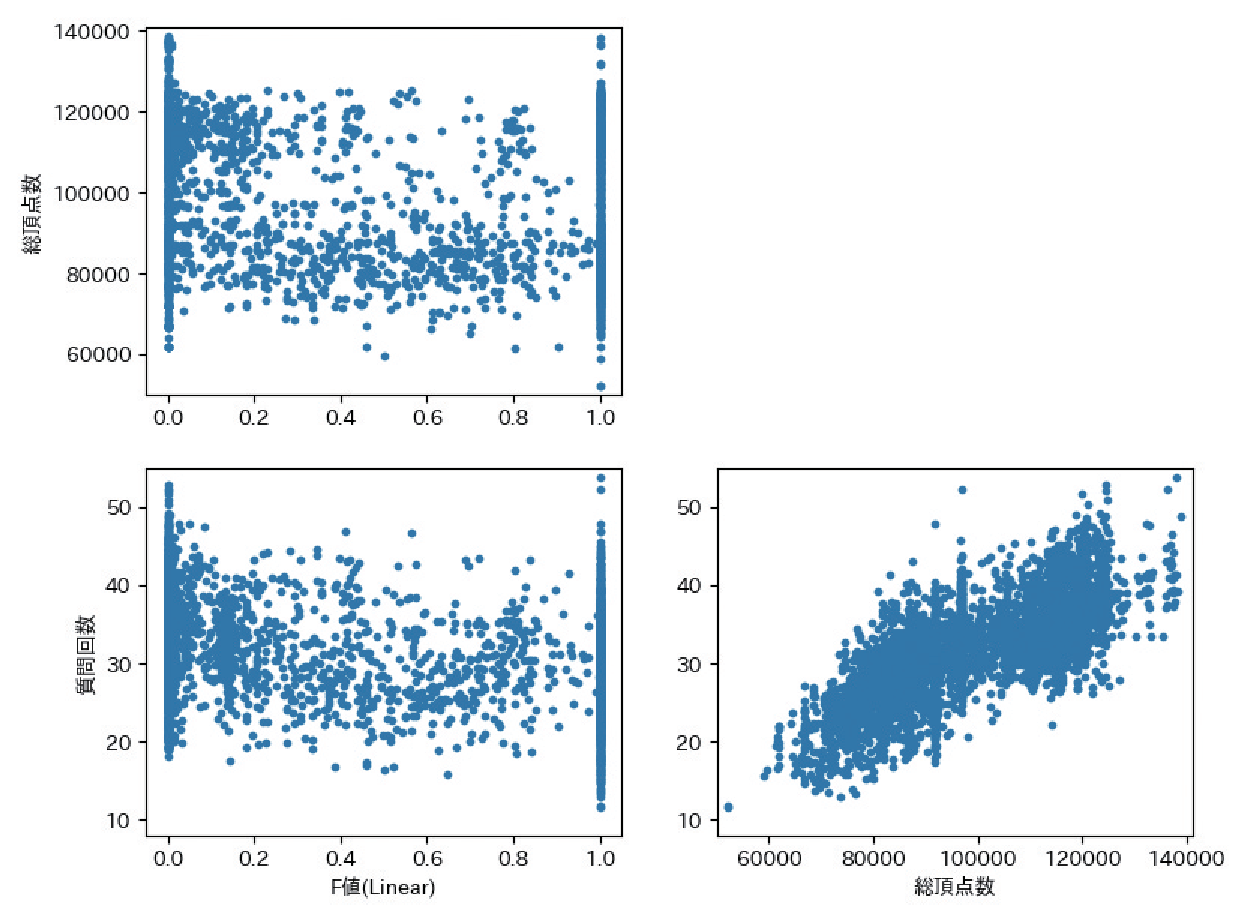
\includegraphics[scale=0.66]{fig-GraphConv_ln_ql_f1_nodes.eps}
  \caption{グラフ畳み込み層にGraphConvを,質問学習アルゴリズムに${\cal LUTP}$-${\cal QUERY}_{GCN^S}^{Linear}$を使用し,F値と質問回数と無順序木パターンの正例の総頂点数による解析結果}\label{fig:GraphConv_ln_ql_f1_nodes}
\end{figure*}

% 図4.7
\begin{figure*}[tb]
  \centering
  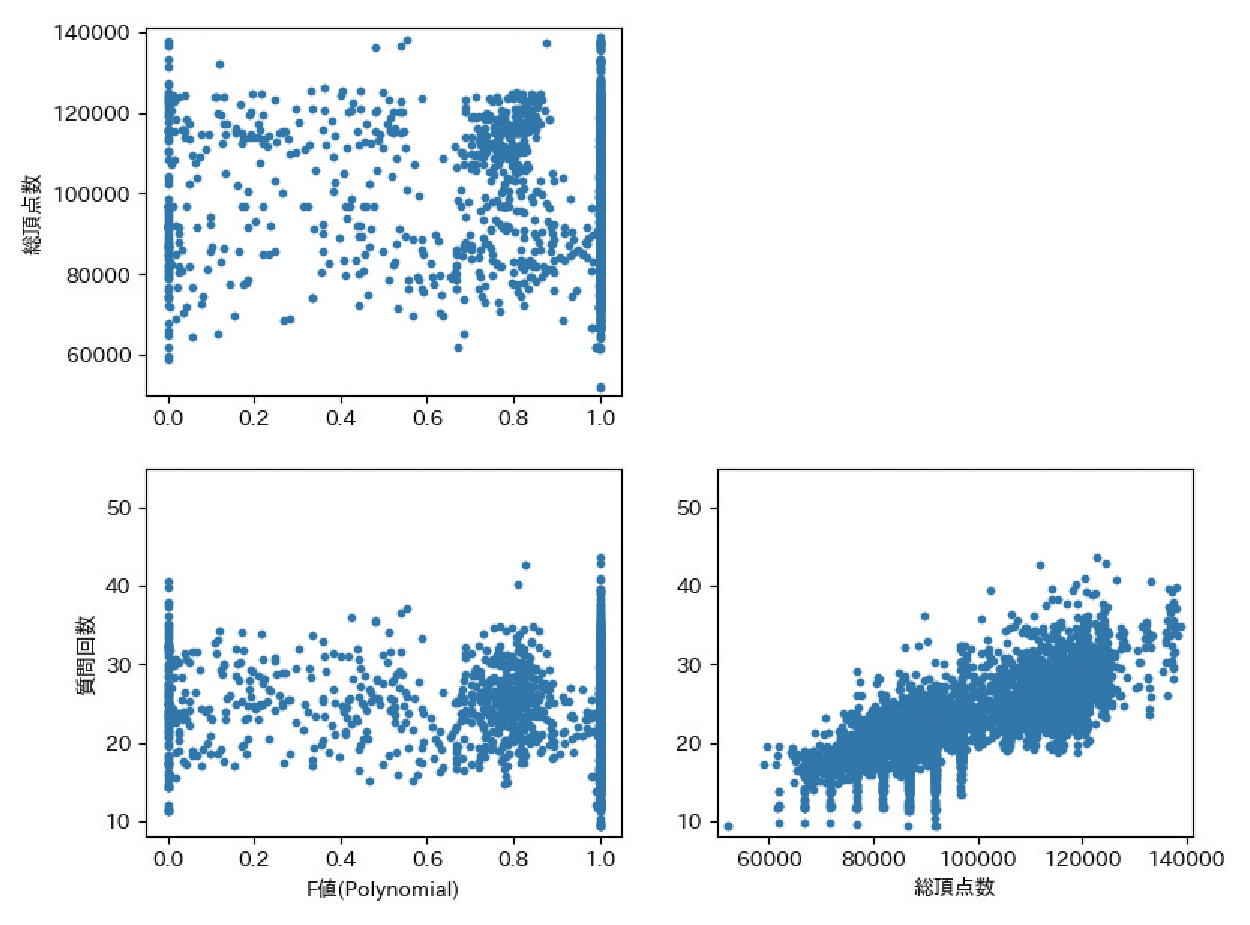
\includegraphics[scale=0.66]{fig-GraphConv_sqr_ql_f1_nodes.eps}
  \caption{グラフ畳み込み層にGraphConvを,質問学習アルゴリズムに${\cal LUTP}$-${\cal QUERY}_{GCN^S}^{Square}$を使用し,F値と質問回数と無順序木パターンの正例の総頂点数による解析結果}\label{fig:GraphConv_sqr_ql_f1_nodes}
\end{figure*}

% 図4.8
\begin{figure*}[tb]
  \centering
  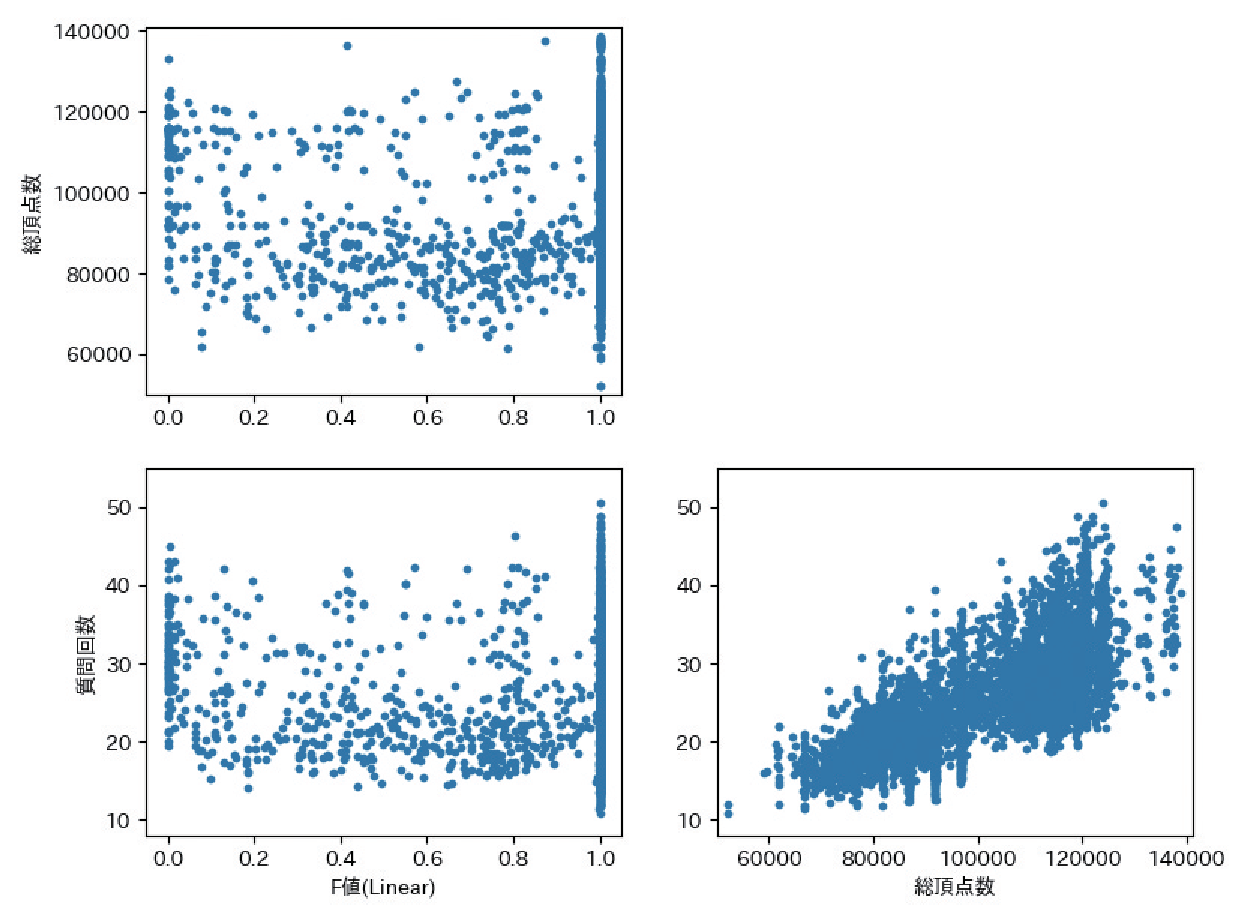
\includegraphics[scale=0.66]{fig-RGCNConv_ln_ql_f1_nodes.eps}
  \caption{グラフ畳み込み層にRGCNConvを,質問学習アルゴリズムに${\cal LUTP}$-${\cal QUERY}_{GCN^S}^{Linear}$を使用し,F値と質問回数と無順序木パターンの正例の総頂点数による解析結果}\label{fig:RGCNConv_ln_ql_f1_nodes}
\end{figure*}

% 図4.9
\begin{figure*}[tb]
  \centering
  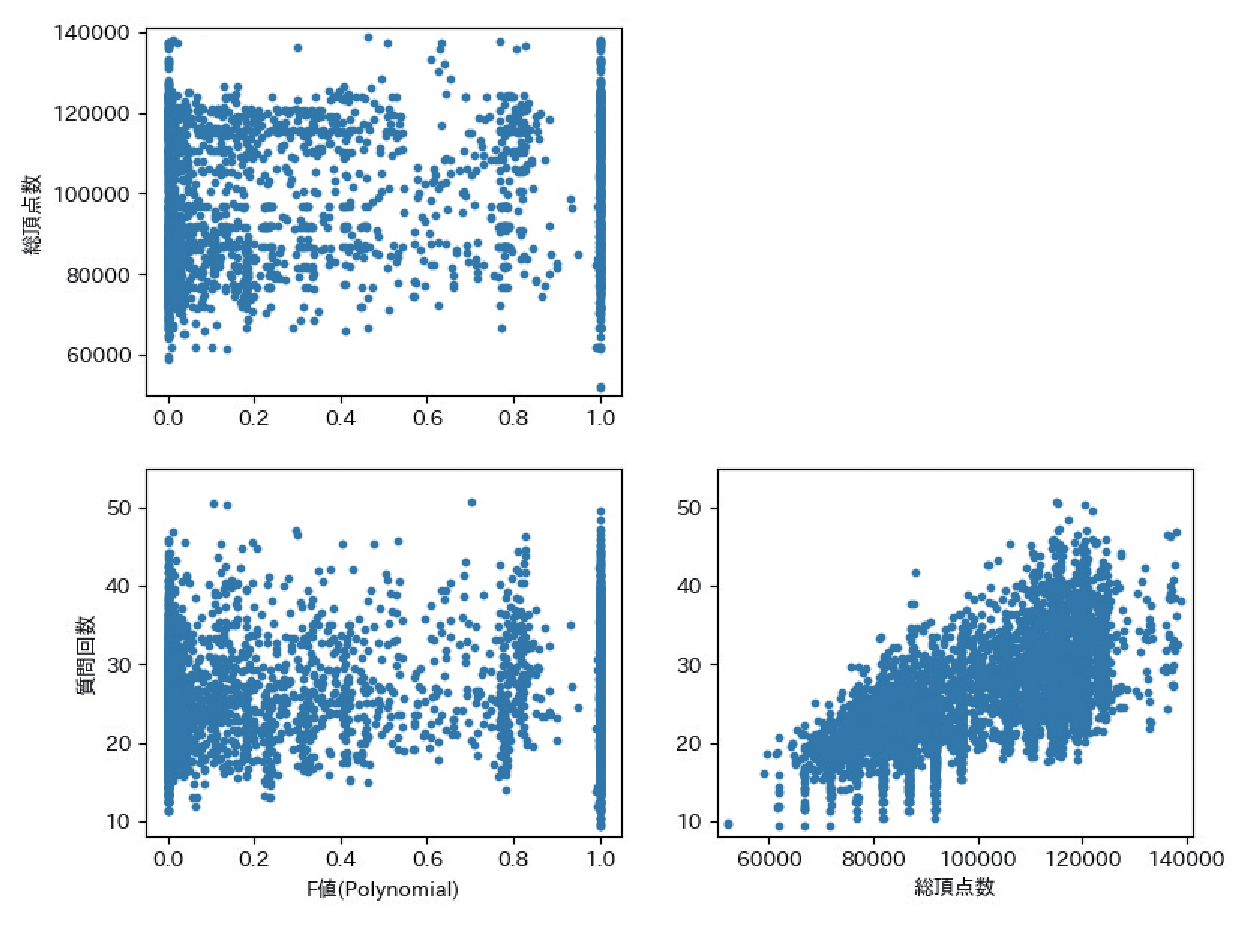
\includegraphics[scale=0.66]{fig-RGCNConv_sqr_ql_f1_nodes.eps}
  \caption{グラフ畳み込み層にRGCNConvを,質問学習アルゴリズムに${\cal LUTP}$-${\cal QUERY}_{GCN^S}^{Square}$を使用し,F値と質問回数と無順序木パターンの正例の総頂点数による解析結果}\label{fig:RGCNConv_sqr_ql_f1_nodes}
\end{figure*}

% 図4.10
\begin{figure*}[tb]
  \centering
  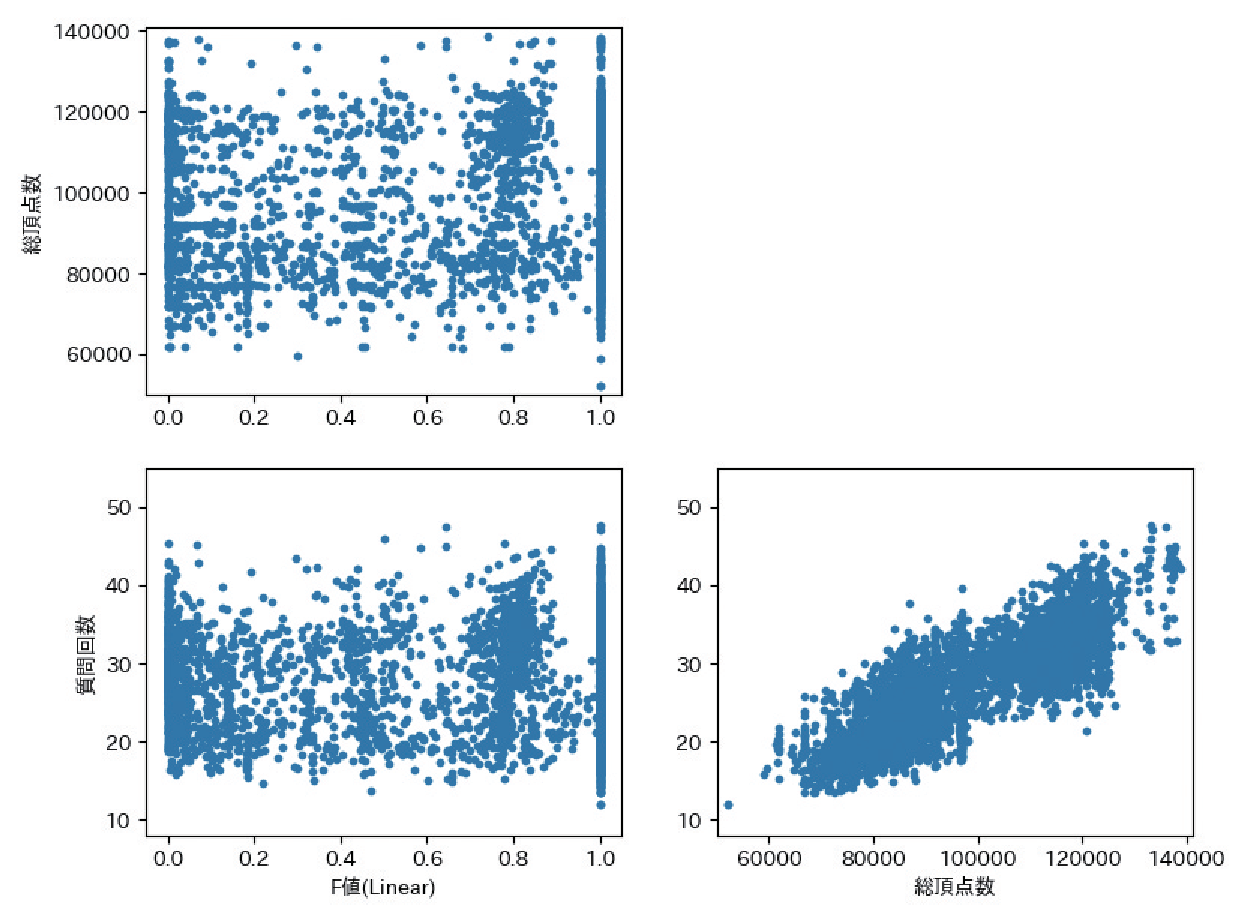
\includegraphics[scale=0.66]{fig-GCNConv_ln_ql_f1_nodes.eps}
  \caption{グラフ畳み込み層にGCNConvを,質問学習アルゴリズムに${\cal LUTP}$-${\cal QUERY}_{GCN^S}^{Linear}$を使用し,F値と質問回数と無順序木パターンの正例の総頂点数による解析結果}\label{fig:GCNConv_ln_ql_f1_nodes}
\end{figure*}

% 図4.11
\begin{figure*}[tb]
  \centering
  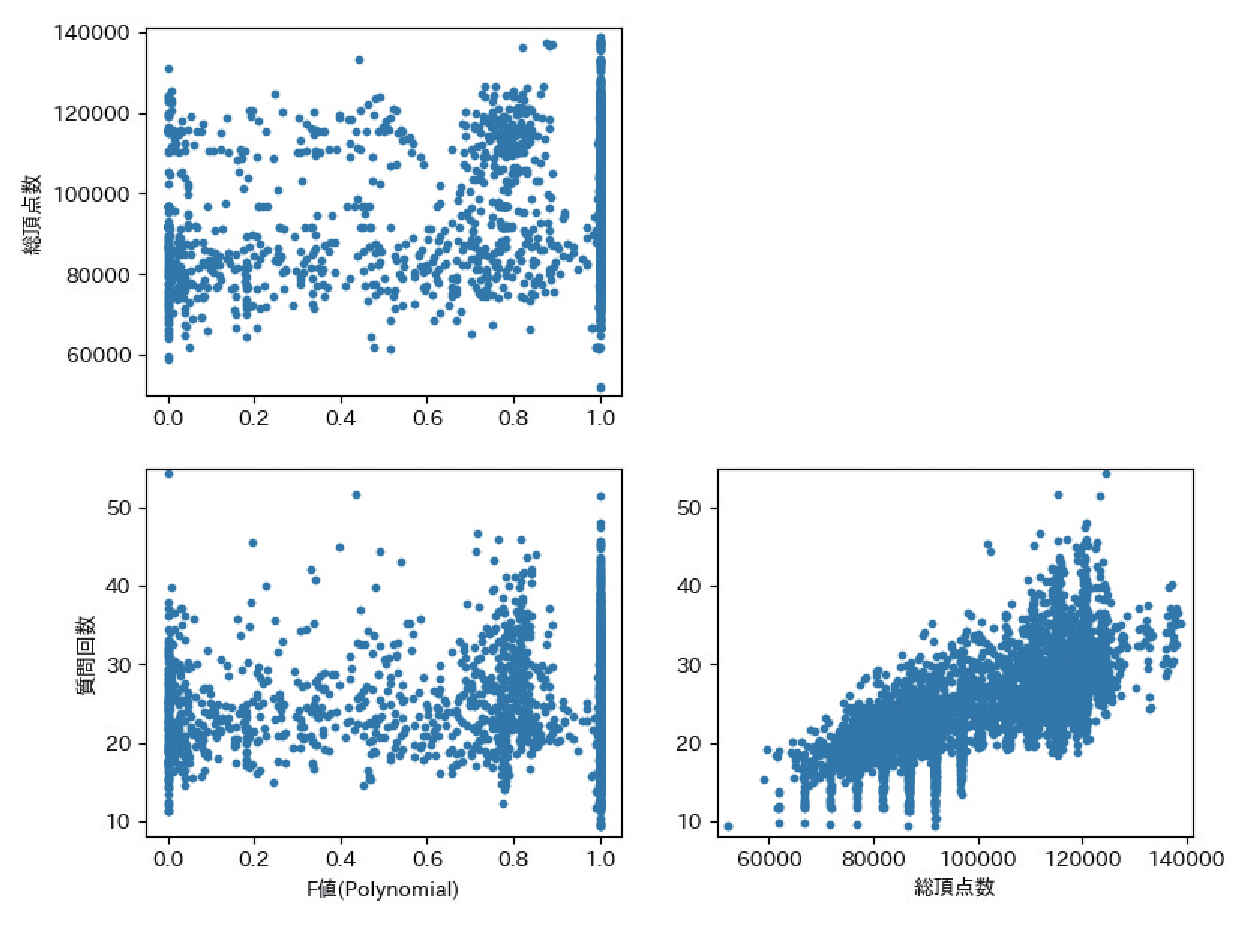
\includegraphics[scale=0.66]{fig-GCNConv_sqr_ql_f1_nodes.eps}
  \caption{グラフ畳み込み層にGCNConvを,質問学習アルゴリズムに${\cal LUTP}$-${\cal QUERY}_{GCN^S}^{Square}$を使用し,F値と質問回数と無順序木パターンの正例の総頂点数による解析結果}\label{fig:GCNConv_sqr_ql_f1_nodes}
\end{figure*}


% Step1:変数の数を特定する
%\begin{step}{\bf 変数の数を特定する}\par
%  \begin{enumerate}
%  \item $d:=h$;
%  \item 深さ$d$の全ての葉$v$に対して,次を行う:\\
%    \hspace*{3truemm} 辺$(p(v),v)$を変数$[p(v),v]$とみなし,$P_{h-d+1}$を束縛して,無順序木$T'$を作成する;\\
%    \hspace*{3truemm} {\bf if} $\mathcal{O}(t_{\ast})(T')=Yes$ {\bf then} $T:=T'$;
%  \item 深さ$d-1$にある全頂点$v$に対して,次を行う;\\
%    \hspace*{3truemm} $v$の子を$c_1,\ldots,c_n(n\geq 2)$とする;\\
%    \hspace*{3truemm} $C:=\{c_i\mid T[c_i]\equiv P_{h-d+1}(1\leq i\leq n)\}$;\\
%    \hspace*{3truemm} {\bf for} $c$ {\bf in} $C$ {\bf do}\\
%      \hspace*{6truemm} {\bf if} $|C| > 1$ {\bf then}\\
%        \hspace*{9truemm} $C$から$c$を削除する;\\
%        \hspace*{9truemm} $T$から$T[c]$を削除して,無順序木$T'$を作成する.ただし,$c$と$p((c),c)$も一緒に削除する;\\
%      \hspace*{6truemm} {\bf if} $\mathcal{O}(t_{\ast})(T')=Yes$ {\bf then} $T:=T'$;
%  \item {\bf if} $d>1$ {\bf then} $d:=d-1$; \\
%        {\bf togo} 2 {\bf else output} $T$;\\
%  \end{enumerate}
%\end{step}

% Step2:最小正例を求める
%\begin{step}{\bf 最小正例を求める}\par
%  \begin{enumerate}
%  \item $d:=1$;
%  \item 深さ$d$の全ての頂点$v$に対して,次を行う:\\
%    \hspace*{3truemm} {\bf if} $T[v]\equiv P_{h-d+1}$ {\bf then}\\
%      \hspace*{6truemm} $T$から$T[v]$を削除して,無順序木$T'$を作成する.ただし,$v$と$(p(v),v)$は削除しない;\\
%      \hspace*{6truemm} {\bf if} $\mathcal{O}(t_{\ast})(T')=Yes$ {\bf then} $T:=T'$;
%  \item {\bf if} $d<h$ {\bf then} $d:=d+1$;\\
%        {\bf togo} 2 {\bf else output} $T$;
%  \end{enumerate}
%\end{step}

% Step3:変数を特定する
%\begin{step}{\bf 変数を特定する}\par
%  \begin{enumerate}
%  \item {\bf if} $T$の根が子を持つ {\bf then}
%  \end{enumerate}
%\end{step}